\paragraph{Navigation Camera}
\label{navigationCamera}

The Navigation camera(Navcam) is a mast-mounted stereo pair of engineering cameras which are seperated by a baseline lenght of 42.4cm. They are designed to survey the terrain around the rover by acquiring images from atop a pan/tilt mast mounted on the top deck of the rover with a $360\degree$ field of the terrain. It is located at the RSM head, co-boresighted with the Mast Camera.
\begin{figure}[H]
	\centering
	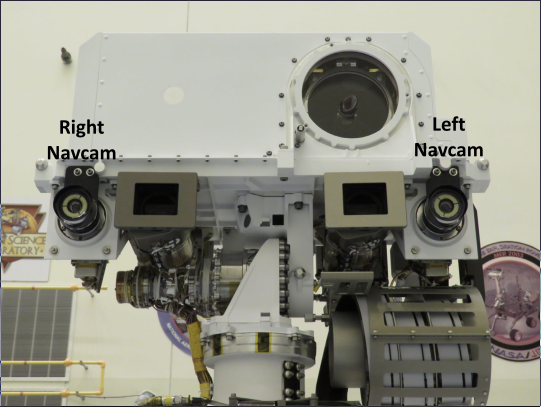
\includegraphics[scale=0.5]{img/locationNavcams.png}
	\caption{Navcam Location}
	\label{fig:navcamLocation}
\end{figure}
The Navcam images are used for traverse planning, general site characterization(panoramic images and targeted images of interest, including terrains that are not viewable by the Hazard Avoidance Camera), target identification and selection, robotic arm operation and rover auto-navigation. The Navcams are also used to monitor and document the state of the vehicle by acquiring images of the rover harware and determine the rover attitude in the local Mars frame by acquiring images of the sun. The label of the images taken by Navcam starts with 'NL' and 'NR' identifiying the left and the right Navcam images. 

\begin{table}[H]
	\centering
	\caption{Navcam Characteristics}
	\label{tab:navcamChar}
	\begin{tabular}{ | p{5cm} | p{5cm} | } 
  \hline
  Optics                             & Description\\
  \hline
  Horizontal FOV                     & 96\degree\\
  Vertical FOV                       & 73\degree \\
  Diagonal FOV                       & 120\degree \\
  Focal Ratio                        & $f/12$\\
  Best Focus                         & 3.5 meters\\
  Stereo Baseline                    & 42.4$m$\\
  Angle between left/right boresight & $<0.4\degree$(parallel)\\
  Boresight mounting orientation     & Mounted to pan/tilt RSM, left/right camera boresights are parallel.\\
  Height above nominal surface       & approx. 1.98 meters viewing the horizon.\\
  Pixel Format                       & 5120 x 3840\\
  Pixel pitch                        & 6.4 \textmu m x 6.4 \textmu m\\
  Optical format                     & Full frame(32.77 mm x 24.58mm)\\
  \hline
	\end{tabular}
\end{table}

\paragraph{Mast Camera Zoom}
\label{mastCameraZoom}

The Mastcam-Z is a multispectral, stereoscopic imaging investigation device on the Mars 2020 mission's Perseverance rover. Each Mastcam-Z camera consists of a 1648 x 1214 pixel charge-shift detector and electronics, in addition to zoom, focus and filter wheel mechanisms. The two Mastcam-Z cameras are mounted on a rover reconnaissance mast with a 24.4 cm stereo baseline and have a total 2.3\degree toe-in on the camera plate approximately 2m from the surface that provides azimuth and elevation triggers. 
\begin{figure}[H]
	\centering
	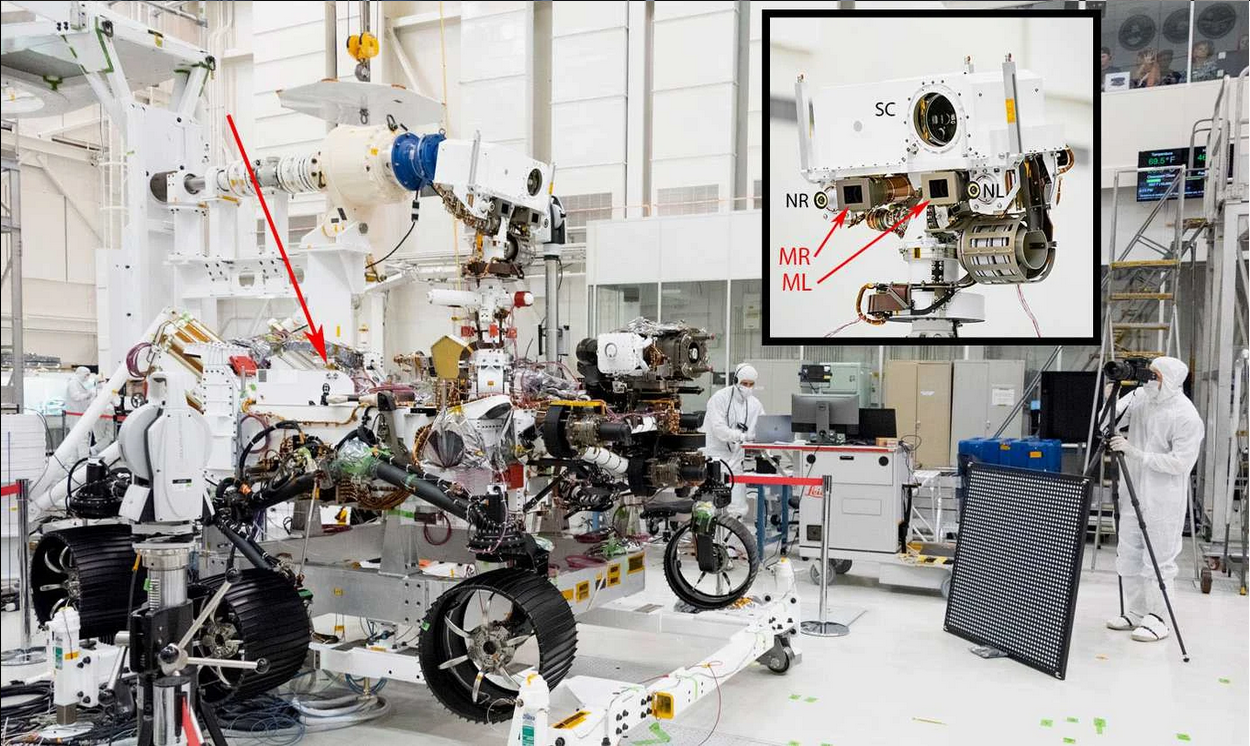
\includegraphics[scale=0.3]{img/mastcamlocation.png}
	\label{fig:mastcamLocation}
	\caption{Location of MastcamZ}
\end{figure}
Primary and secondary MastcamZ calibration targets mounted on the rover's upper deck allow for tactical reflectance calibration. It uses Mastcam-Z's multispectral, stereo and panoramic imagery to provide detailed morphological, topographical and geological context along the rover's traverse. Limit the mineralogical, photometric and physical properties of surface materials. Monitoring and characterization of atmospheric and astronomical phenomena. Document rover sample extraction and cache locations. Mastcam Z images  also provide important technical information to support sample selection and other rover drive and tool equipment operation decisions.

\begin{table}[H]
	\centering
	\caption{Mastcam Characteristics}
	\label{tab:mastcamChar}
	\begin{tabular}{ | p{5cm} | p{5cm} | } 
  \hline
  Optics                 & Description\\
  \hline
  Focus                  & Adjustable, Working distance $0.5-1.0 m to \infty$ \\
  FOV(1600 x 1200 pix)   & 25.6\degree x 19.2\degree Widest and 6.2\degree x 4.6\degree Narrowest\\
  Focal ratio            & f/6.7 and f/9.5\\
  Effective focal length & 26 mm and 110 mm\\
  Array size             & 1600 x 1200 photoactive pixels ( 1648 x 1214 total)\\
  Pixel size             & 7.4\textmu (square pixels)\\
  Stereo baseline        & 24.4 cm; toe-in angle between cameras; 2.3\degree\\
  \hline
	\end{tabular}
\end{table}




%Refernce
%
%[1]https://pds-geosciences.wustl.edu/m2020/urn-nasa-pds-mars2020_mission/document_camera/Mars2020_Camera_SIS.pdf
%
%[2]https://www.vrvis.at/publications/pdfs/PB-VRVis-2021-025.pdf)
%
%[3][mastcam](https://link.springer.com/article/10.1007/s11214-020-00755-x)


%[2]improvment of the cameras from the MSL in the perseverance rover.
%Navcam FOV was too narrow, limited assement of the vehicle state due to the lack of color information
%lower angular pixel scale
